\section{Experimental Setup}
\label{sec:experimental-setup}

\section{Modelagem e Análise de Hierarquias de Cache}
\label{sec:mechanism}

Consideramos hierarquias de cache dentro de uma rede de borda/nuvem representada como DAGs. As caches são substituições acionadas a cada cache que são ativadas para atender os usuários. Essa aproximação é baseada no rastreamento de um objeto atingido em um cache pai de volta a uma chegada correspondente.

A Figura 3 ilustra o cenário abordadoneste trabalho. Aqui, nós consideramos uma topologia em árvore binária com sete nós e um \textit{Cloud Provider} conectado ao nó raiz. Os últimos quatro nós são pontos de acesso~(AP) e os outros são pontos de peering de borda. Os nós AP são implementados em dispositivos sem fio que se comunicam via IEEE 802.11g em 2,4 GHz. Os APs têm conexões com fio para os pontos de peering de borda, enquanto os usuários finais também são sem fio. Cada usuário conectado ao AP está localizado a precisamente 8 metros de distância do AP. A largura de banda disponível é de 20Mbs nos links 0-1 e 0-2; e 30Mbs nos links 1-3, 1-4, 2-5 e 2-6.

\subsection{Abordagem de Decomposição}

O objetivo geral do nosso design é melhorar a QoE dos usuários de download de conteúdo, que se caracteriza principalmente pela latência do conteúdo e pela taxa de download. 
Apresentamos três estrategias que abordam os impactos identificados na Seção III na rede multicamada de borda/nuvem, ou seja, \textit{Only-Cloud}, \textit{QoS-Greedy} e \textit{ILP Solution}. 

O cenário \textit{Only-Cloud} usa apenas o nó Provedor de Nuvem para entregar o conteúdo de vídeo. Por outro lado, a abordagem \textit{QoS-Greedy} usa os nós da rede de borda, sempre que um congestionamento de link é detectado o \textit{QoS-Greedy} é ativado para escolher qual nó da borda para auxilar na entrega do vídeo.   A simulação começa com os usuários solicitando o vídeo da nuvem. Quando um link congestionado é detectado, o cache de borda abaixo do link é ativado. A partir daí, os usuários que recebem o vídeo pelo link congestionado são redirecionados para os nós de borda 1 e 2.


\subsection{Avaliação de QoE}

Dentre os modelos existentes na literatura, nós descrevemos como as metricas de QoE podem ser usadas para pontuar a satisfação do usuário. Primeiramente, cada pedaço de qualidade de vídeo é calculado por uma lei logarítmica sobre taxas de bits. A equação 1 mostra a transformação numérica da qualidade do video recebida pelo usuário. Cada vídeo tem $N$ segmentos e é codificado com $L$ níveis de taxa de bits. $r_i$ representa um nível de taxa de bits específico. A cada passo $i$, a qualidade do segmento $i$ é definida.

\begin{equation}\label{eq:equation-1}
q(r_i) = a_1 * log(a_2 * (r_i/ r_{L}))
\end{equation}
\vspace{0.1cm}

Para calcular a satisfação de cada usuário no longo prazo, é necessário um modelo flexível que inclua as métricas mais influentes para quantificar a QoE dos usuários. Consideramos a Equação 2 de [12], que consiste em quatro métricas: (a) a qualidade perceptual média do pedaço, (b) o número médio de oscilações de qualidade, (c) o número médio de eventos de estol e sua duração, e (d)) o atraso de inicialização. $K$ representa o total de segmentos do vídeo, $S_i$ é a duração da parada e $ST_i$ é o atraso de inicialização do usuário $i$.

\begin{equation}\label{eq:qoe-equation}
\begin{split}
QoE_i = \frac{1}{K} \sum_{k=1}^{K}q(r_{k}) - \frac{1}{K-1} \sum_{k=1}^{K-1}|q(r_{k+1}) - q(r_{k})| - \frac{1}{K}\sum_{k=1}^{K} S_{k} - ST_{i}
\end{split}
\end{equation}
\vspace{0.1cm}

O $QoE_{i}$ para cada usuário $i$ pode variar de 1 a 5, onde 1 = ruim, 2 = ruim, 3 = regular, 4 = bom e 5 = excelente.

\begin{figure}[htb!]
    \centering
    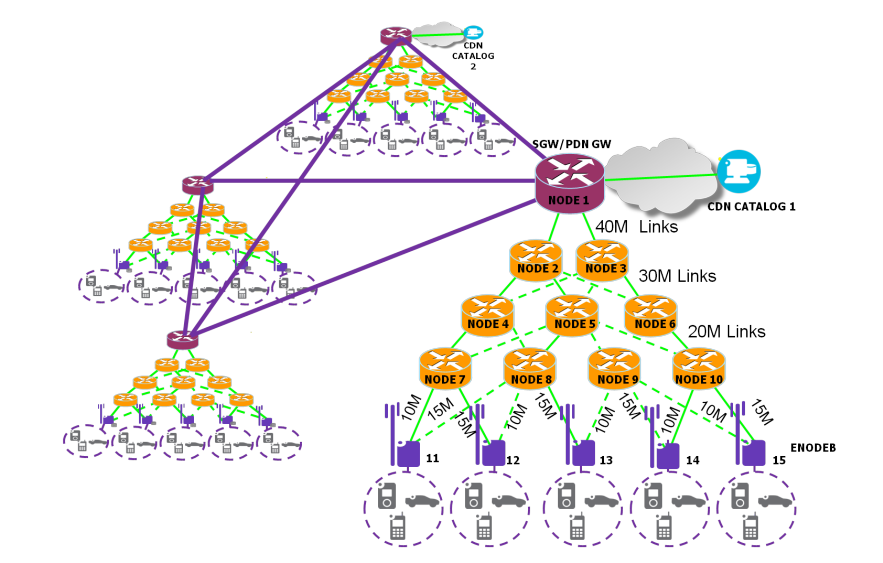
\includegraphics[width=\linewidth]{images/scenario.png}
    \caption{A General Overview of the multi-tier network environment.}
    \label{fig:multi-tier-network}
\end{figure}

